\documentclass[12pt,letterpaper]{report}
\usepackage{natbib}
\usepackage{geometry}
%\usepackage{fancyheadings} fancyheadings is obsolete: replaced by fancyhdr. JL
\usepackage{fancyhdr}
\usepackage{afterpage}
\usepackage{graphicx}
\usepackage{amsmath,amssymb,amsbsy}
\usepackage{dcolumn,array}
\usepackage{tocloft}
\usepackage{asudis}

\begin{document}
%-----------------------front matter
\pagenumbering{roman}
\title{Challenge Task 2018}
\subtitle{Implementation of a Decentralized Application Tic Tac Toe}
\paperType{Dissertation}
\chair{Departements of Informatics - Communication Systems Group}
\memberOne{Lucas Pelloni, leginumeber}
\memberTwo{Severin Wullschleger leginumber}
\memberThree{Andreas Schaufelbühl, 12-918-843}

\maketitle
\doublespace
%\include{abstract}
\dedicationpage{}
%\include{ack}
\tableofcontents
% This puts the word "Page" right justified above everything else.
\addtocontents{toc}{~\hfill Page\par}
% Asking LaTeX for a new page here guarantees that the LOF is on a separate page
% after the TOC ends.
\newpage
% Making the LOT and LOF "parts" rather than chapters gets them indented at
% level -1 according to the chart: top of page 4 of the document at
% ftp://tug.ctan.org/pub/tex-archive/macros/latex/contrib/tocloft/tocloft.pdf
\addcontentsline{toc}{part}{LIST OF TABLES}
\renewcommand{\cftlabel}{Table}
\listoftables
% This gets the headers for the LOT right on the first page.  Subsequent pages
% are handled by the fancyhdr code in the asudis.sty file.
\addtocontents{lot}{Table~\hfill Page \par}
\newpage
\addcontentsline{toc}{part}{LIST OF FIGURES}
\addtocontents{toc}{CHAPTER \par}
\renewcommand{\cftlabel}{Figure}
\listoffigures
% This gets the headers for the LOF right on the first page.  Subsequent pages
% are handled by the fancyhdr code in the asudis.sty file.
\addtocontents{lof}{Figure~\hfill Page \par}
%-----------------------body
\doublespace
\pagenumbering{arabic}
\chapter{Introduction}\label{ch:introduction}
%introduce to the task and idea
This years \ac{ct} is to implement a \ac{dapp}  running in the Ethereum blockchain. The goal of the application is a playable Tic-Tac-Toe\footnote{https://en.wikipedia.org/wiki/Tic-tac-toe} game, which also includes a betting system, all embedded in a \ac{sc}.
\\\\
%Introduce more our project here

Chapter \ref{ch:technologies} gives an overview and short explanation of the technologies we use in order to implement the \ac{ct}.\\
In Chapter \ref{ch:implementation} we show the actual implementation of the game. It starts by explaining and showing our project structure. Also we give walk-through of the different processes of playing a game and betting on games.\\
The problems and challenges occurred within our project are discussed in Chapter \ref{ch:discussion}. Additionally we also describe our open task and goals for the future concerning this project.
\chapter{Technologies}
%which technologies are used and why

\chapter{Implementation of the game}\label{ch:implementation}
\section{The Smart Contract}
\noindent The diagram in Figure\ref{fig:sc_uml}  shows a detail structure explaining the modelling of our \ac{sc}. \\
\begin{figure}[ht]
	\begin{center}
		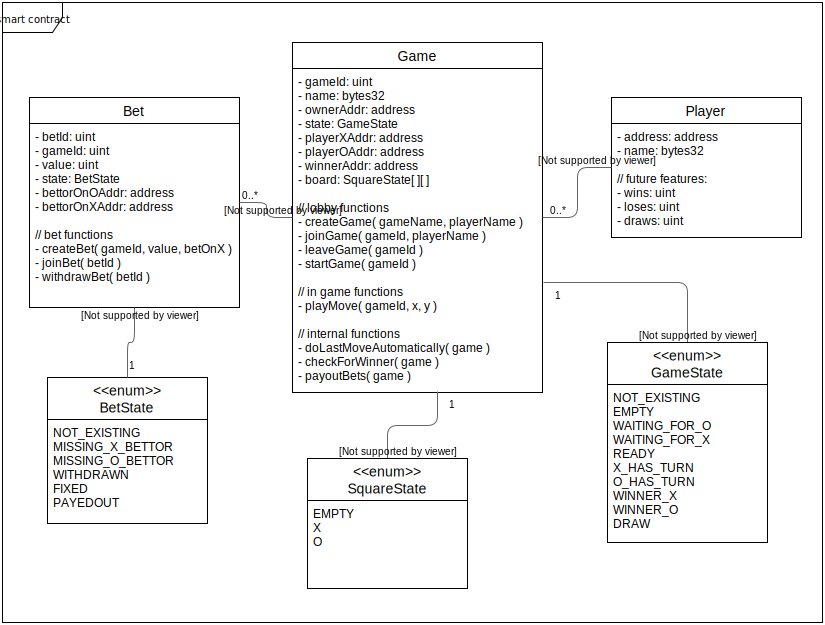
\includegraphics[scale=0.22]{res/sc_uml}
	\end{center}
	\caption{Structure of the \ac{sc}}
	\label{fig:sc_uml}
\end{figure}\newline
\noindent The \ac{sc} can hold multiple games, which always contain one board and two players. Every time a user opens up a new Game, he automatically gets assigned as one of the playing party. Now the Game state is automatically set to 'WAITING\_FOR\_X'. As soon as a second player chooses to enter a open game, the game-owner can start the game, which changes the state to 'X\_HAS\_TURN' as the game has now started and the guest player has to do his first move.\\\\
All Bets contain a game-id pointing to a game which the bet is referencing on it. The user who creates a bet chooses the game and the amount of token he wants to bet with and pays it into the \ac{sc}. Is there an opponent bettor joining the bet, the state changes to 'FIXED'.\\
If the game finds an end, the state of it changes to either 'WINNER\_X', 'WINNER\_O' or 'DRAW', which activates the function 'payout' ,triggering all bets referencing to this particular game. So the bets will change the state to 'PAYOUT' and user will get paid according to their betting.\\ 
Three functions of the \ac{sc} we show here, to discuss in detail the implementation and structure of the \ac{sc}:\\





%logic and modell

\chapter{Discusion}\label{ch:discussion}
\section{Challenges and Problems}
\section{Future work}
%logic and modell
\include{chapter5}
\include{chapter6}
%-----------------------back matter
{\singlespace
% Making the references a "part" rather than a chapter gets it indented at
% level -1 according to the chart: top of page 4 of the document at
% ftp://tug.ctan.org/pub/tex-archive/macros/latex/contrib/tocloft/tocloft.pdf
\addcontentsline{toc}{part}{REFERENCES}
\bibliographystyle{asudis}
\bibliography{dis}}
\renewcommand{\chaptername}{APPENDIX}
\addtocontents{toc}{APPENDIX \par}
\appendix
\include{appendix1}
\include{vita}
\end{document}
